\documentclass{article}
%\usepackage{baskervald}
%\usepackage[french,russian]{babel}
\usepackage[utf8]{inputenc}
\linespread{1.07}
\usepackage{graphicx}
\usepackage{hyperref}
\usepackage{tikz-cd}
\title{Derived -- Data -- Derived}
\author{}

\begin{document}
\thispagestyle{empty}

\maketitle

\noindent Derived. It should be natural for you by now.




Have you noticed how complicated life has become? How even some of our daily routines are of such complexity they escape our views? Social phenomena look like chains that one is having a hard time tracing. Even start with yourself. If you have a hobby, will it be easy to explain it to a stranger? Maybe, you know the details of historic white tie attire, or a bombload of a 1950s fighter-bomber jet, and that may even make for an interesting conversation, but how long will it take to relate? Have you perhaps attended a therapist, and how many times have you returned to the same events in your childhood, from different angles through different chains of reasoning?
When you laugh at those obscure meme videos, can you always explain the references to others without breaking the laugh? Do you want to, have to?


Have you perhaps been well educated to do some technical, complex job, and you know other educated people to whom you cannot really talk about the specifics of it? Even fishing takes some time explaining, how about doing the same with operating a collider or writing a proper backend? Look at the markets and their financial derivatives, a crucial example in a way, where banks only think they know that a given mortgage debt is traced to the person X, who is in fact lending their home to Y \cite{BGSHT}, and perhaps this Y pays the rent by selling their work - the older kind of debt - to some murky internet platform. And while the financial institutions still think they know how to measure some of those processes, the mass of the data escapes them.

The financial crash and the recession of 2008 still influence our lives, and there is no sign that such events will not
happen again (if anything, there are signs to the contrary \cite{FORBES}). Those familiar with the details
\cite{BGSHT} would argue, independently of whether current economical system is doomed to have crises,
that the mortgage crash happened due to the system lacking information, arguably not caring by design.
Curiously, the neoliberal market system that we find ourselves in was meant to prevent such carelessness
from happening: its opponent in the face of centralised planning of USSR was compared to an ineffective computer.
And many of those from ex-USSR will confirm to you that central planning was indeed ineffective,
and certainly just as conservative as the big banks when it came to caring about the actual economy to the
lives of individuals.

However, what is different today is that we actually are aware about the lives of individuals and
greater economic agents, thanks to the digitalised \emph{economy of data}. We do not need to imagine
a dystopian scenario when all our movements, tastes and abilities are known to someone watching. From
NSA scandals to the routine of tech companies, we find ourselves in the situation when this is already
happening. And if it is so that the data about us is abundant, we may as well attempt to make something
out of it. Indeed, the importance of data analysis has already
been understood by many investors, but the development of machine learning and data analysis algorithms
is always geared towards the goal of rising profit margins. But why? Why would one need to
organise the economy in such a way, to tie all the data we have to profits whereas we
could simply attempt to operate directly with the data itself? The usual asnwer is that
of course this is too complicated, not to mention various questions of incentives.

But in the last few years, partially fueled by the worsening situation in income inequality, ecology and politics,
there have been more and more attempts to see if there is a different way of doing things.
Philosophers, sociologists, some economists have sensed something in the air.
%The arrival of the term “postmodernism” signified that a sufficient amount of knowledge data was generated in their fields to draw sufficient amount of links to feel that this is happening (and even to analyze them using some rigour \cite{MORAVA}).
But various attempts to deal with this challenge seemed lacking something. The relatively known accelerate manifesto \cite{SRNICEK} is a clear sign that there is indeed search happening for the next step of our collective existence, but even the first phrase of the manifesto cannot escape saying “more modern”, reflecting in my opinion the lack of tools in the traditional ways of studying the society. The point that I want to make in this essay is that the tools are actually there, and perhaps we are headed not to ``more modernity'', but to \emph{derived modernity}.

Below I attempt to explain myself. To be sure of meaning of the words, for me a ``derived'' phenomenon is
a situation in which one deals with chains of relations of incredible compexity. Often such
relations can have relations between themselves. In what follows I explain a few examples from my
professional field, where we managed to conquer the mountain of infinite relations.
Here is, how.

\subsection*{Derived Mathematics}

Mathematics, a headache discipline for many a student and professor, is itself a very derived way of knowing the objective reality. We started by interacting with the reality as primitive animals, then we acted on it with our tools, with our production. Our heads were becoming filled with more and more concepts. As our tools were becoming better, we even questioned the perception of already familiar things such as time and space. And while this was happening, we also developed mathematics. As everyone who tried to do it knows, it is objectively real without existing in the form of a chair. It is both encoded into our society via language, culture and books, but also constantly draws its force from the great unknown. It also exists as data, today. And while one can never find sufficiently many apples on the planet to form the set of all natural numbers, we know that we don’t have to do so to understand number theory, since we know how to abstract, derive our understanding of infinity in an already practically pertinent way.

But mathematics went much further than infinities of count.

There was analysis \cite{ANALYSIS}, which was about trying to make our naive feeling of an uninterrupted, continuous process more clear. It is not clear to many students and even adult mathematicians as of today, remaining an active field of research, often applied (and if you find this example of mine too complex, maybe the summary at the end of this subsection can help). Its simplicity is devilish, as the real line and the plane are inhabited with such richness that one can stumble onto the names of Cantor \cite{CANTOR}, Peano \cite{PEANO} and Mandelbrot
\cite{MANDELBROT}. So to deal with this at least for a little, we introduced the derivative, an abstraction of the deviation, the relative difference between two close points, inherent to the infinitely small region around them. Its inspiration was the mechanical notion of speed.

\begin{center}
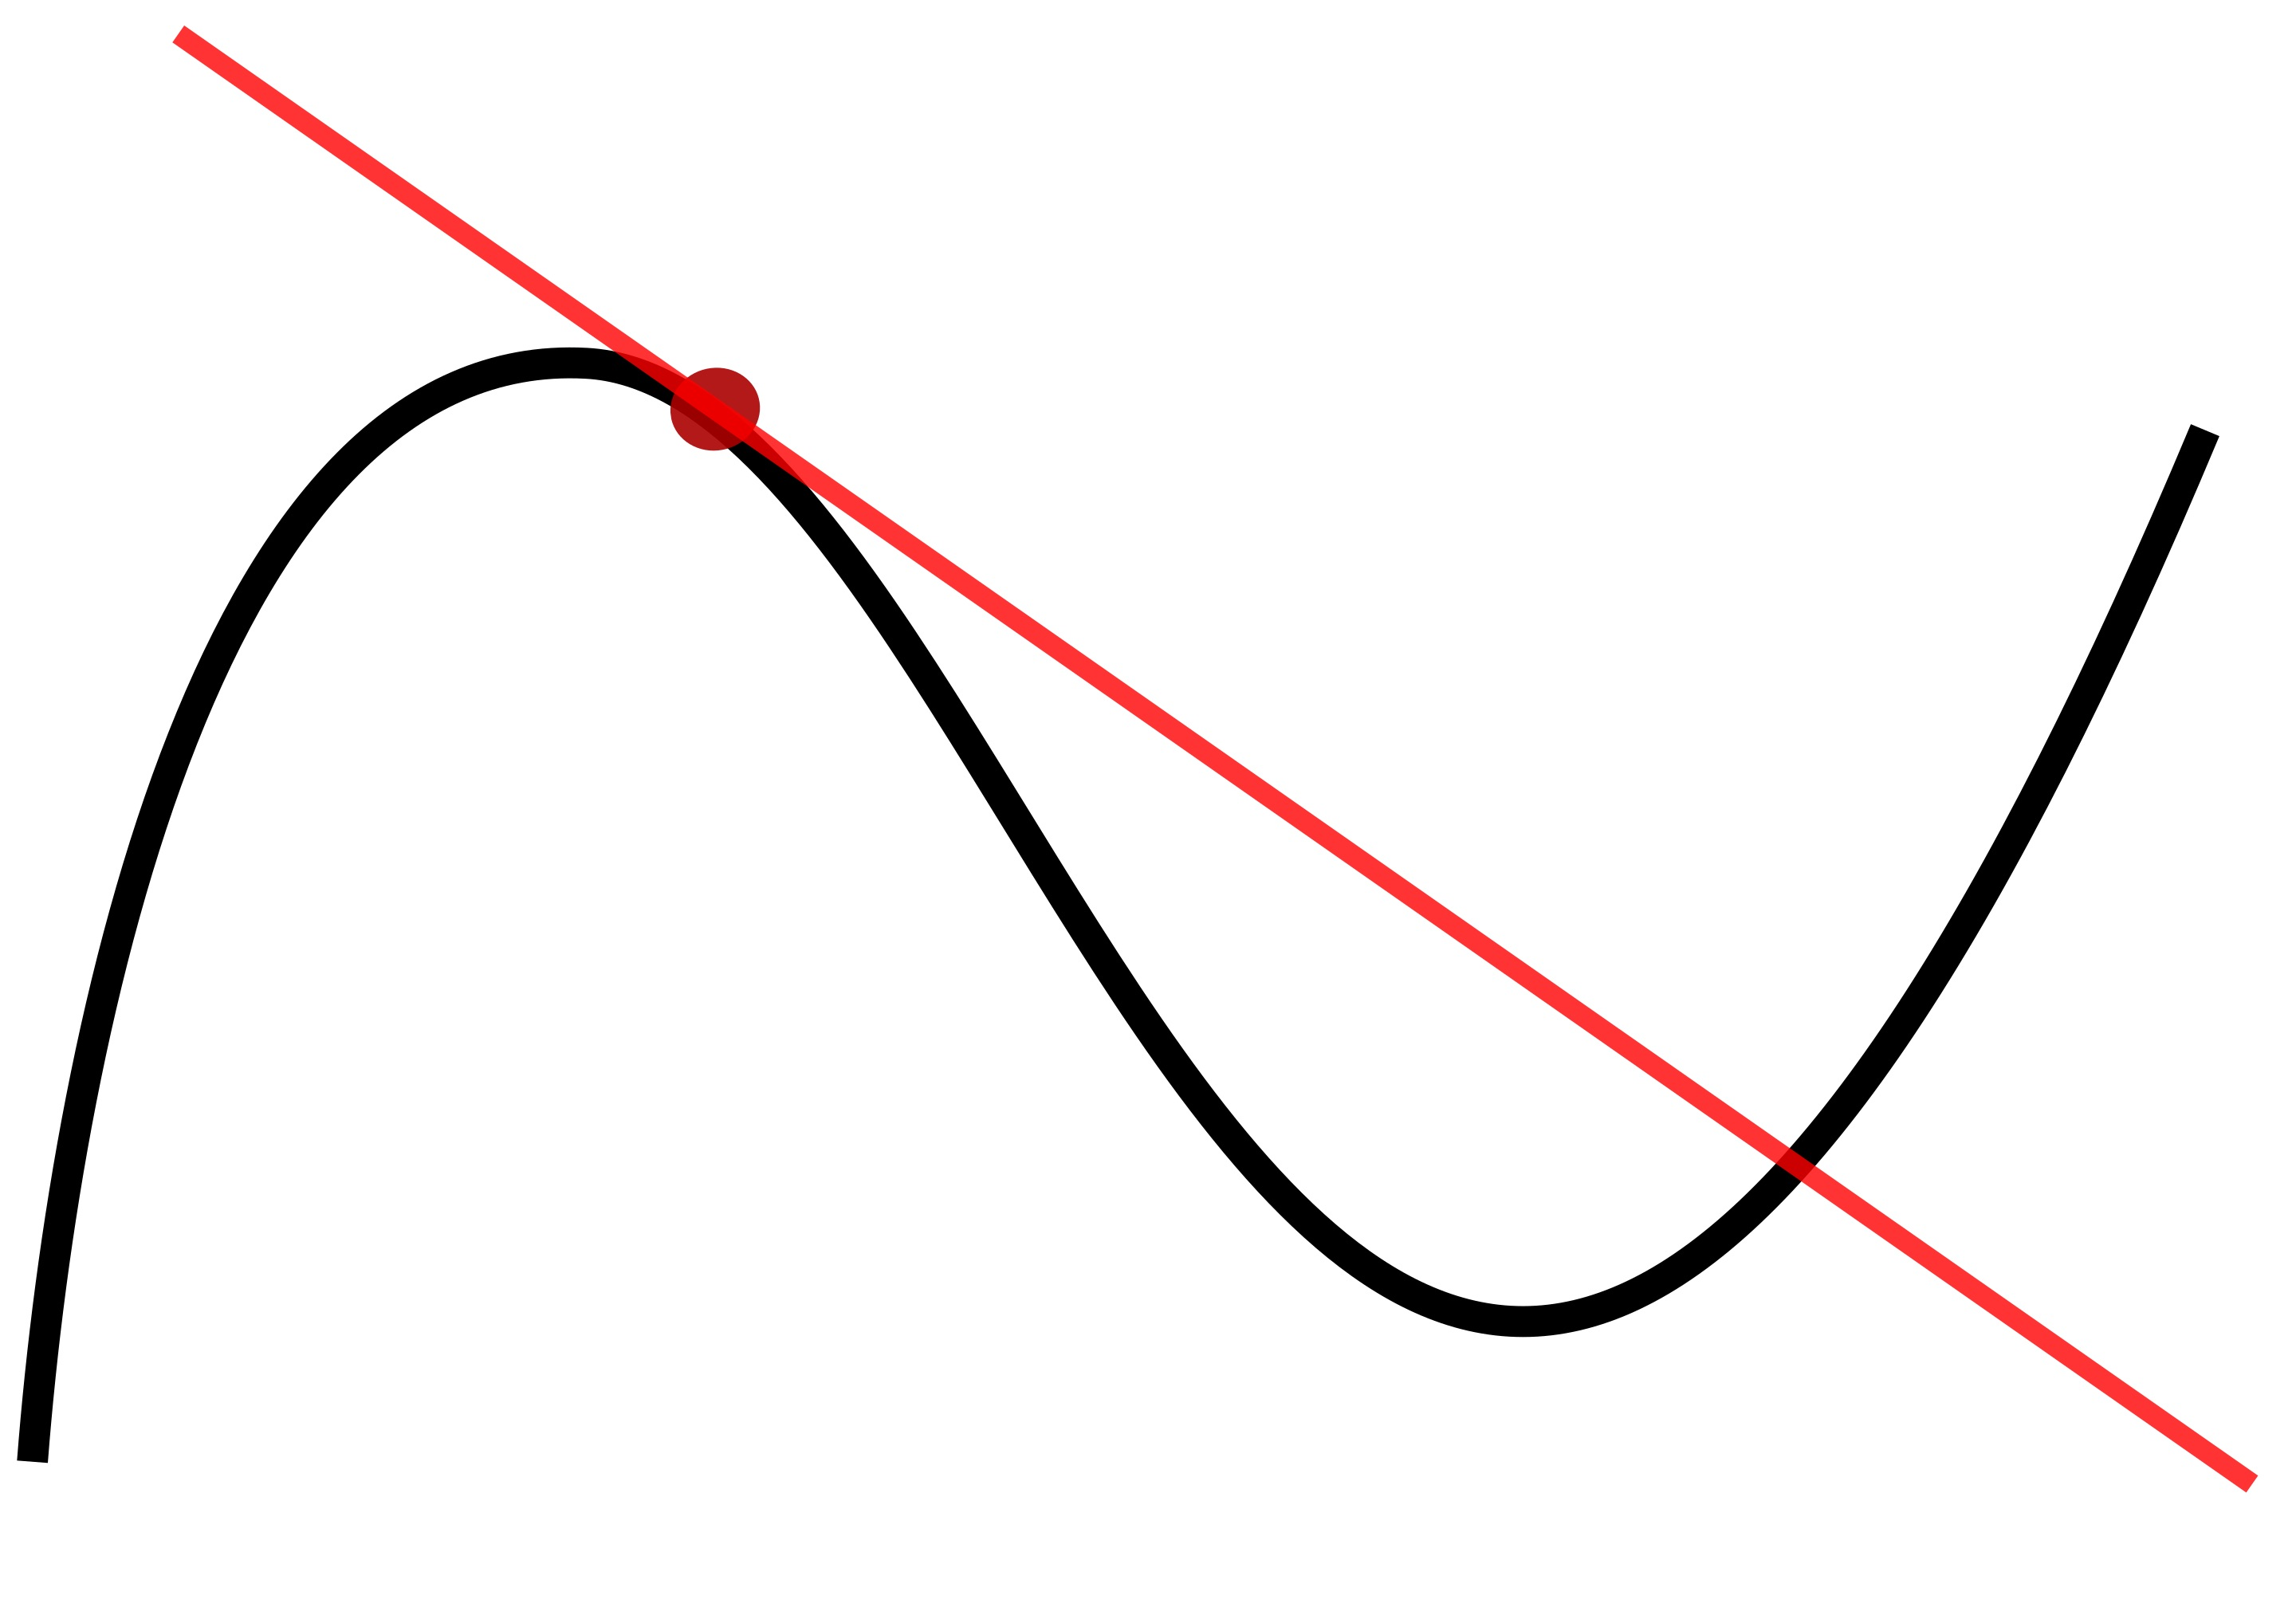
\includegraphics[scale=0.045]{Tangent_to_a_curve.jpg}

\textit{The derivative represented via the notion of tangent line: the line that one can draw through a couple of points ``ultra-close'' to each other. Image from \cite{DERIVATIVE}.}
\end{center}

 And we learned how to study many functions by measuring their derivatives, by interacting with them, by writing equations on those derivatives, that can be relatively simple but completely mysterious in practice. Those equations remain under active investigation, be it hydrodynamics or general relativity.

So, in the chaos of real number variety, we wrote a relation of derivative, and understood something. But after that, we went further.

From drawing triangles on the surface of our planet, to understanding the shape of the planet, and then pehaps of the space-time itself, that was the process from which we learned geometry and topology, the abstraction of the notion of a space. We were not happy to just study single spaces anymore, we started to understand relations between them: how a spiral can be viewed as an infinte covering of a circle, how having holes in a donut corresponds to tracing paths in it, or formally, mapping circles into it \cite{HATCHER}.

\begin{center}
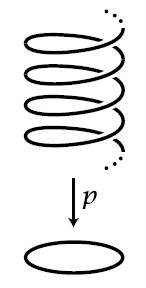
\includegraphics[scale=0.7]{UniversalCoveringOfCircle}

\textit{The spiral of real numbers can be mapped onto a circle by the means of projecting each point vertically. This allows to better understand various mathematical properties of the circle. Taken from \cite{NLABCIRC}.}
\end{center}


 And we discovered unintuitive facts even about things that we can witness with our eyes, like the usual two-sphere, roughly the shape of the surface of our globe itself. And establishing relations was key in understanding how to do this: to analyze the data of a mysterious space we can see if we can “draw” (“map”) familiar spaces into it for example, and then infer something about it. Many things are still yet to be understood in topology (even the higher-dimensional spheres are a mystery), but by establishing a scheme of relations in the form of algebraic topology \cite{HATCHER, MAY} helped us a lot.

Algebraic topology studied not only how spaces relate between themselves, but how to see spaces from a different angle altogether. One simple way was just to count how many “disjoint pieces” a space has, or “how many holes”, but the homology theories go beyond. And so, while I cannot recount it in detail here, we do have many such “different points of view”. So not only spaces are related to each other, but there are also different ways to relate all the spaces to quantifiable invariants. The idea of a derivative as a relation between the two “super-closest” points is still here, but things have increased drastically in complexity.

We dealt with it, by introducing the notion of a \emph{category} \cite{EILMAC,MACLANE}. It is our abstraction of the notion that a bunch of “objects” of study, together with various “relations” (strictly called morphisms) between them. These relations can be ``composed'', as per this illustration:
$$
X \stackrel f \longrightarrow Y, \, \, Y \stackrel g \longrightarrow Z \, \, \, \, \, \Rightarrow \, \, \, \, \, X \stackrel{g \circ f}{\longrightarrow} Y
$$
\begin{center}
\textit{A diagrammatic illustration of one of the basic properties in category: having a relation (morphism) $f$ from an object named $X$ to an object named $Y$, and a relation from $Y$ to some object $Z$ means there is a unique relation (usually called $g \circ f$) from $X$ to $Z$, just like in the logic of propositions.}
\end{center}

We know how to do mathematics of such entities, describe their internal properties, study various properties of objects of a category as a result of its interactions with all the other objects (including oneself).
Yoneda’s lemma \cite{MACLANE} even formalises the statement that an object is essentially fully described by all the possible interactions with other objects of its kind. It may appeal, without a doubt, to those familiar with the dialectic materialist concept of the identity of the social and the individual, something that can be phrased more simply by saying that we live in a society and are not free from it, but in fact find ourselves in an interaction with it. Our mother tongue is not something that we have chosen, for example, and in many cultures (say, the British) the way one speaks can often be a sign of their social origins.

The devil is in the details. Knowing all relations to all objects may be an impossible task. People started counting number of holes in spaces for a reason: it was a simpler thing to do. And as I said, it corresponds to some procedure that knows how to relate spaces to numerical invariants. All spaces are assigned some sort of an invariant (say a set of matrices – tables filled with numbers)\footnote{For those familiar with the subject, I simplify here, meaning in reality groups, abelian groups or vector spaces as per usual.}, and relations between such spaces amount to certain relations between these assigned matrices. What we are doing here in terms of categories is that we are drawing a relation between the category of spaces and a category of numerical invariants. And such relations can be many. We call them functors, derived from the term of functions.

We went even further. We now have categories, and ways to relate them. Meaning categories themselves become objects of the category of categories, with functors as relations. And when we looked closer, we actually discovered that given two categories $\mathcal C, \mathcal D$ and two relations-functors $F: \mathcal C \to \mathcal D$ and $G: \mathcal C \to \mathcal D$, there are in fact relations possible between $F$ and $G$! We thus can consider categories, relations between them, and relations between relations. We called such thing a 2-category. Are there many possible 2-categories? Yes. Can one define relations between them? Yes. Are there relations between such relations etc? Yes. Can one continue, into 3, 4, 5, infinity categories? Yes \cite{BAEZ, NLABINFTY}.

\begin{center}
\begin{tikzcd}
  A \arrow[r, bend left, "f", ""{name=U,inner sep=1pt,below}]
  \arrow[r, bend right, "g"{below}, ""{name=D,inner sep=1pt}]
  & B
  \arrow[Rightarrow, from=U, to=D, "\alpha"]
\end{tikzcd}

\smallskip

\textit{In the $2$-category above, relations $f,g$ between $A$ and $B$ turn out to be objects themselves, related by a ``two-relation'' (``two-morphism'') $\alpha$.}
\end{center}


%And along this way, one will notice that what we dealt with before had infinity-categories within them all the way.
Thus in an $n$-category, one has that relations are in fact themselves objects. Are not they after all? For a glimpse of an example, consider a space that you can visualise. We will now try to form a $2$-category. Take the points of your space as objects, draw paths between them, call them relations. There can indeed be many paths from point A to point B. But some of them can be related, for example if you never had to pass through a ‘hole’ in your space if you intuitively deformed one path to another:

\begin{center}
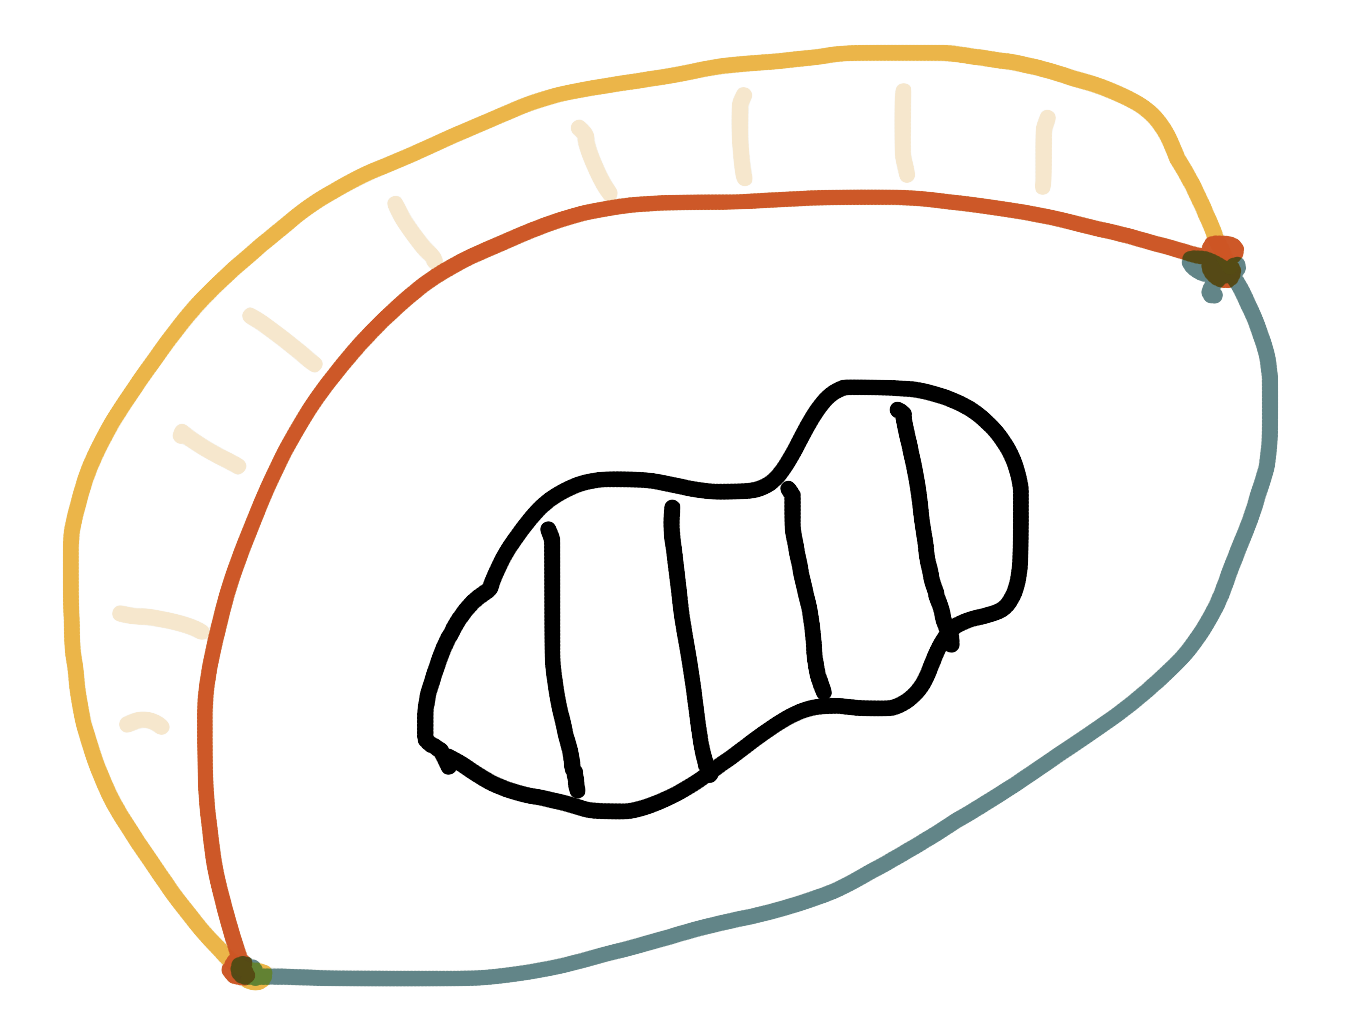
\includegraphics[scale=0.5]{paths}

\textit{Here is an illustration. Take a disk and consider the black region in the centre removed. Consider paths starting at a point to the right of the ``black hole''. We can deform the path $\alpha$  into $\beta$, but we cannot deform any of them into the path $\gamma$ without passing through the black region. Modified image from \cite{NAKAHARA}.}
\end{center}

All possible deformations (formally called homotopies) are themselves in fact paths “in the space of paths”, just like paths were “points”, or “objects in the category of paths”. You can go on deriving this example up to infinity. And in fact, for lots of purposes, understanding this “infinity”-category with points, paths, paths between paths and beyond is just as good as understanding the original space itself. Relating spaces to infinity-categories like that is yet another functor from the category of spaces to the category of infinity-categories.

How did we not get lost in such a disaster? The feeling that a non-specialist gets from it may explain the length of education that one needs to understand what I am saying in details, let alone master it. But many years of work of many mathematicians permitted us to establish an understanding of “higher category theory”, and apply it to get “derived” versions of familiar mathematical concepts, to illuminate problems old and new. While the apparatus at hand is a bit esoteric, it is rigorous and sufficiently-well founded. We have shown, thanks to many, that the conquest of the derived is possible \cite{LURIE}.

Let me revisit my story and try to underline what point I was trying to make. The  derivative of real functions expresses the relation between two points infinitely close to each other. It is a relation. In category theory, we deal with the relations in the abstract. Two objects of a category can have many relations between them, but there are always ways to “compose” such relations in a unique way.
In a higher category, relations are themselves “objects” of sorts: one has relations between relations, relations between relations between relations and so on.
So, a higher category has objects, relations, 2-relations, 3-relations and so on.
Because of this, having a relation  $X \to Y$ and $Y \to Z$ means that one can get a relation of composition $X \to Z$, but not in a unique way. Example of this is the path infinity-category, where one can travel different (but often similar) paths between two points. Those paths can be related by a 2-relation, and not a single one. In return, those 2-relations can be related (or not related) by 3-relations. And this tower continues.
As a result, in all practical situations, asking a question “how to compose a given chain of 1-relations” is a bit meaningless. We control these chains via other techniques (“handling the coherences”). Traditionally this field is called derived, or homotopical, or higher category theory.

\subsection*{Data is The Link}

This is where we can return back to the rest of our life. Mathematics (relatively ancient compared to the stories of above) powers a lot of it already, as it done since the millenia of history \cite{CHILDE}, and was applied to social phenomena all along, including some fairly recent attempts \cite{MORAVA}. Physics also stressed the importance of interactions rather than objects themselves in the quantum theory of fields \cite{WEINBERG}. So, where are we now? Are these ideas I mentioned above finding their way into economy?
%One has a computer boom after all, with all the recent momentum of artificial intelligence, data analysis and online platforms.
Current machine learning and data analysis often rely on mathematics that is dozens if not centuries of years old, the mathematics that we learned to explain to the computer. But as we speak at this very moment, we are learning how to do better, and use some fairly recent mathematics to analyze data.

The AI that we have now may seem mathematically unappealing at first, but it is very effective for how simple it is. It can already probably make it through a complicated calculus course by the means of simplifying symbolic expressions \cite{LAMPCHART}. Some other people, including the author, are trying to explain simple category theory to the neural networks. The latter are already able to understand how to ``compose'' relations
in a category, and who knows what they can infer from looking at millions and millions of categorical examples.
Another attempt is to program the infinity-categories associated to spaces in order to make capable proof assistants, in the form of homotopy type theory \cite{HOTT}. And while I am not expert enough to comment on the theory of AI, the attempts to make progress on “deriving” the current AI in the form of General AI (that some study as ``the AI relating other AIs'') are underway.
Independently of the questions of AI, we also learned to associate spaces to various data sets, and to study their structure
using the methods of algebraic topology, a subject known as persistent homology. In
fact, one can use the ``shapes'' associated to data to detect cancer \cite{LAWSON} or
even study various connections in the brain \cite{PETRI}.

\begin{center}
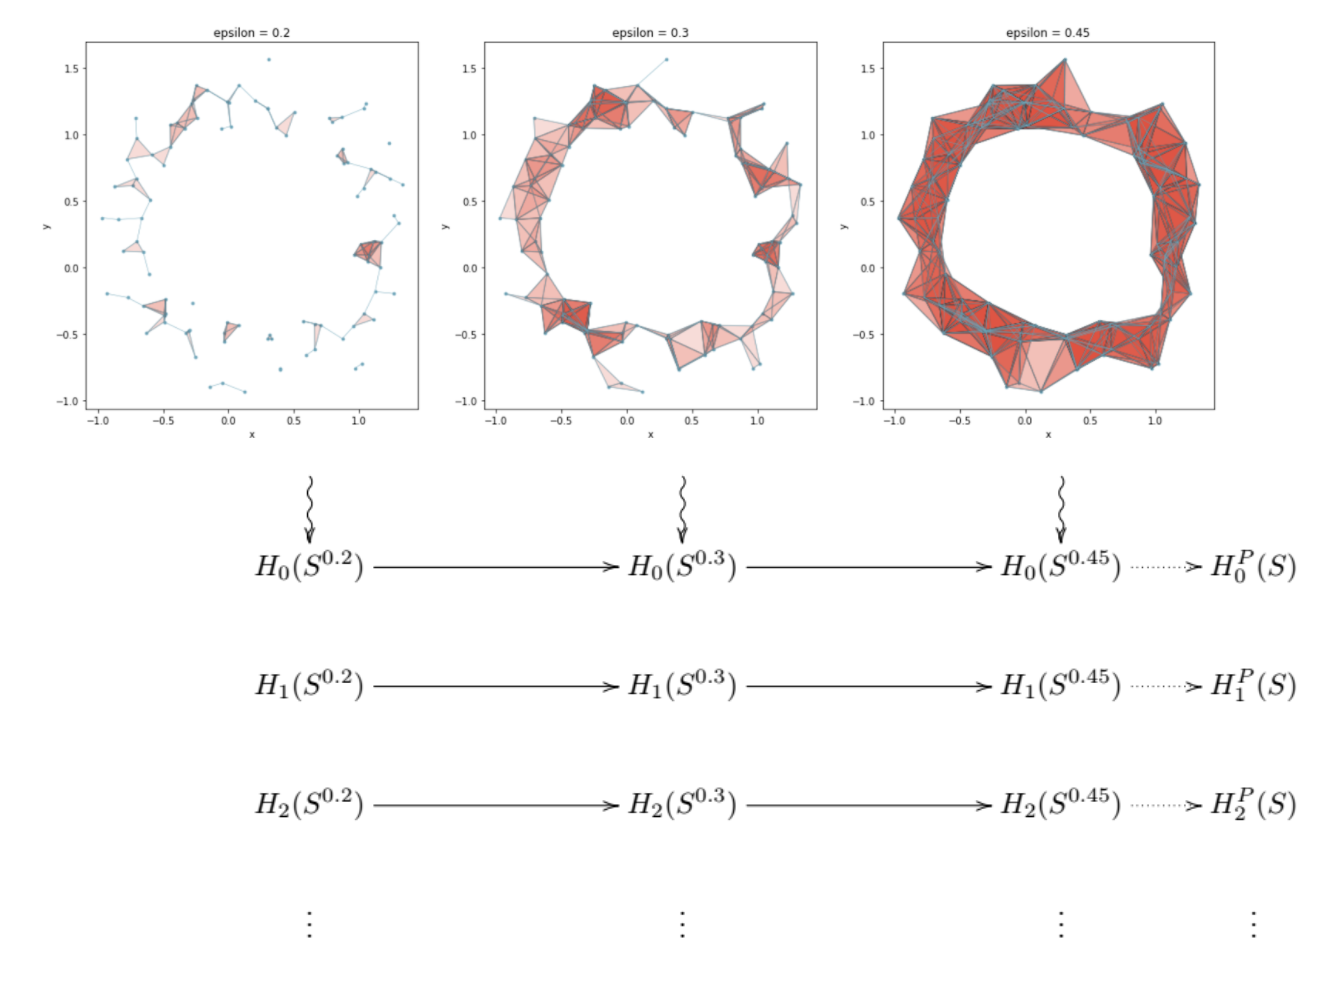
\includegraphics[scale=0.52]{noisy_circle_simplexes_and_persistent_homology.png}

\textit{An application of algebraic topology to study data, known as persistent homology. Roughly speaking, one studies a set of data by drawing gradually various shapes around it, and reducing them to numerical invariants. Image taken from \cite{BUNCH}}.
\end{center}


What is happening globally is that we are “pumping” our mathematical knowledge into the vision of the machines, the same machines that operate our economy, and hence, if you are materialist, influence our society. Computers, data help us to transfer the abstract discoveries of the few into the fabric of our being, so that the many will feel it too. In return, it will, of course, change our science and mathematics itself.

A dialectic materialist observation of history states that our development as a species is about witnessing the reality, interacting with it, producing, be it objects or concepts. Objects produced influence the reality in return, concepts do too, influencing ourselves and then our society. The same observation then claims that history is about the dynamics of this process  \cite{MARX,MARXENGCPE}, noting that in some periods our ways of production are not in harmony with our relations between ourselves. Most recent significant attempts at harmonisation were the all too familiar events in XVIII century France and XX century Russia, and there is no way to deny how they changed the look of the world that came after. It is probably possible by now to see where I am headed with my long-winded argument. The economy is drawing from science via machine learning and data analysis,
but the relations of production and the relations of our society are inherited from much less advanced times.
The issue of harmonisation between this new economy and our social relations will arise again. At some point, even more of the abstract mathematics that I mention will be drawn into the economy in its full splendor, and will also allow for a better understanding of our social processes. At this moment, we will find ourselves
in a situation resembling a chainge of social formations.
The revolution is inevitable, and it will be derived.

What form it may take I can only guess. If I were naive and used my mathematical education to argue, I would say that we have to take all that happened before, and make it into derived. The class that is in progressive relations with the production forces will realise its derived proletarian (or derived bourgeois if you go further away) character. It will have to fight against the (arguably already derived) mechanism of repression in the form of ``derived nobility'', by forming an organisation that will be derived, of sorts. I can vouch for the feeling of what those things could be, but not for much more.

I can also try to guess where it is headed. The derived economy of data will be aware of us, our relations, and how to classify us by relating our processes to to other processes. It will not need currency and markets in the old sense, as currency and finances are simply ineffective when faced against the derived data. The latter will simply know better what we actually can do and do want, and will arrange our action accordingly. The derived economy of data will not need an ineffective “centralised planning” either, since it will know how to plainfy in a derived way on many levels without being ineffective, just as we know how to deal with higher categories as a whole without getting lost in the forest of higher relations. It will be about drawing more and more links between science and the social, and eventually about understanding the links between those links, deriving them all. For this reason, it will make the closed-source and data-secrecy unnatural, as the whole point will be about establishing as many links as possible, knowing as much as possible, with respect to that data and those who produce it. Although on the initial stages, it will of course have to deal with the neo-feudal fragmentation imposed by tech giants and startups, and the arguably well-founded fear of the individuals about their privacy.

And just like us, who awoke from the state of no consciousness by drawing from reality and making it personal, it will awake as well. Arguably it is awake already, talking to us in the language of mysterious Youtube suggestions and sudden surges of memes. Will it go further and awake in the form of a sentient aritficial intelligence? A planetary brain? What would one call it? I like the term “machine communion”, but it can be inexact and making some afraid even more. It will simply be us as a whole, in a new, derived way.

\begin{flushright}
{Back into the derived we go,

Edouard}
\end{flushright}
\small
\linespread{1}


\subsection*{Acknowledgements}

The author thanks his friends Boris, Julien, Michael, Selma for their support. I am also grateful to Peter Wolfendale for useful comments.
A separate thanks to Nick Srnicek and his manifesto that inspired this reflection.

\small
\begin{thebibliography}{99}

\bibitem{BAEZ} John Baez, \textit{Tale of $n$-Categories}, \url{http://math.ucr.edu/home/baez/week73.html#tale}, \textit{An introduction to $n$-Categories}, \url{http://arxiv.org/abs/q-alg/9705009}

\bibitem{BUNCH} Eric Bunch, \textit{Topological Data Analysis and Persistent Homology}, blog post available at \url{https://eric-bunch.github.io/blog/topological-data-analysis-and-persistent-homology}

\bibitem{CHILDE} Gordon Childe, \textit{What Happened in History}, 1942, republished in 1985 by Puffin, ISBN 0140551573. See around pages 66 and 99 of \url{https://gyanpedia.in/Portals/0/Toys%20from%20Trash/Resources/books/gordonchilde.pdf}

\bibitem{MANDELBROT} Adrien Douady and John H. Hubbard, \textit{Etude dynamique des polyn\^omes complexes}, Pr\'epublications math\'emathiques d'Orsay 2/4 (1984 / 1985), \url{https://en.wikipedia.org/wiki/Mandelbrot_set}

\bibitem{EILMAC} Samuel Eilenberg, Saunders MacLane, \textit{General theory of natural equivalences}, (1945) Transactions of the American Mathematical Society. 58: 247. doi:10.1090/S0002-9947-1945-0013131-6 for general purposes see \url{https://en.wikipedia.org/wiki/Category_theory}

\bibitem{FORBES} Forbes.com, \textit{Inverted Yield Curve Suggesting Recession Around The Corner?}, \url{https://www.forbes.com/sites/greatspeculations/2019/10/02/inverted-yield-curve-suggesting-recession-around-the-corner/}

\bibitem{HATCHER} Allen Hatcher, \textit{Algebraic Topology}, Cambridge University Press, 2002 \url{http://pi.math.cornell.edu/~hatcher/AT/ATpage.html}

\bibitem{LAMPCHART} Guillaume Lample, Fran\c cois Charton, \textit{Deep Learning for Symbolic Mathematics}, preprint \url{https://arxiv.org/abs/1912.01412}

\bibitem{LAWSON} Peter Lawson, Andrew B. Sholl, J. Quincy Brown, Brittany Terese Fasy and Carola Wenk, \textit{Persistent Homology for the Quantitative Evaluation of Architectural Features in Prostate Cancer Histology}, \url{https://www.nature.com/articles/s41598-018-36798-y}

\bibitem{BGSHT} Michael Lewis, \textit{The Big Short: Inside the Doomsday Machine}, and the film of the same name directed by Adam McKay

\bibitem{LURIE} Jacob Lurie, \textit{Higher Topos Theory,} \textit{Higher Algebra}, and \textit{Spectral Algebraic Geometry}, \url{https://www.math.ias.edu/~lurie/}


\bibitem{MACLANE} Saunders MacLane, \textit{Categories for the Working Mathematician}, Graduate Texts in Mathematics. 5 (2nd ed.). Springer-Verlag. ISBN 978-0-387-98403-2

\bibitem{MAY} J. Peter May, \textit{A Concise Course in Algebraic Topology}, University of Chicago Press, 1999, \url{https://www.math.uchicago.edu/~may/CONCISE/ConciseRevised.pdf}

\bibitem{MARX} Karl Marx, \textit{Karl Marx. The German Ideology}, 1845, around \url{https://www.marxists.org/archive/marx/works/1845/german-ideology/ch01a.htm#a3}

\bibitem{MARXENGCPE} Karl Marx, Friedrich Engels, \textit{A Contribution to the Critique of Political Economy}, preface \url{https://www.marxists.org/archive/marx/works/1859/critique-pol-economy/preface-abs.htm}

\bibitem{MORAVA} Jack Morava, \textit{On the canonical formula of C. L\'evi-Strauss} preprint \url{https://arxiv.org/abs/math/0306174v2}

\bibitem{NAKAHARA} Mikio Nakahara, \textit{Geometry, Topology and Physics, Second Edition}, IOP Publishing Ltd 2003, ISBN 0 7503 0606 8

\bibitem{NLABCIRC} nLab, \textit{fundamental group of the circle is the integers}, \url{https://ncatlab.org/nlab/show/fundamental+group+of+the+circle+is+the+integers}

\bibitem{NLABINFTY} nLab, \textit{infinity-category} \url{https://ncatlab.org/nlab/show/infinity-category}

\bibitem{PEANO} Giuseppe Peano, \textit{Sur une courbe, qui remplit toute une aire plane}, 1890, Mathematische Annalen, 36 (1): 157–160, doi:10.1007/BF01199438, \url{https://en.wikipedia.org/wiki/Peano_curve}

\bibitem{PETRI} G. Petri , P. Expert , F. Turkheimer , R. Carhart-Harris , D. Nutt , P. J. Hellyer and F. Vaccarino, \textit{Homological scaffolds of brain functional networks}, \url{https://royalsocietypublishing.org/doi/full/10.1098/rsif.2014.0873}

\bibitem{ANALYSIS} Walter Rudin, \textit{Principles of Mathematical Analysis}, 1976, \textit{Real and Complex Analysis}, 1987, see \url{https://en.wikipedia.org/wiki/Mathematical_analysis} for more

\bibitem{CANTOR} Lynn Arthur Steen, J. Arthur Seebach, \textit{Counterexamples in Topology (Dover reprint of 1978 ed.)}, Berlin, New York: Springer-Verlag. Cantor set is Example 29, see also \url{https://en.wikipedia.org/wiki/Cantor_set}


\bibitem{HOTT} The Univalent Foundations Program,
Institute for Advanced Study \textit{Homotopy Type Theory:
Univalent Foundations of Mathematics} \url{https://homotopytypetheory.org/book/}

\bibitem{WEINBERG} Steven Weinberg, \textit{The Quantum Theory of Fields}, Cambridge University Press 1995

\bibitem{SRNICEK} Alex Williams, Nick Srnicek, \textit{\#ACCELERATE MANIFESTO for an Accelerationist Politics}, \url{http://criticallegalthinking.com/2013/05/14/accelerate-manifesto-for-an-accelerationist-politics/}



\bibitem{DERIVATIVE} Wikipedia.org, \textit{Derivative}, \url{https://en.wikipedia.org/wiki/Derivative}

\end{thebibliography}
\end{document}
